\documentclass[letterpaper,12pt]{article}
\usepackage[a4paper]{geometry}
\usepackage{amsmath, amssymb, amsthm,graphicx}
\usepackage{fancyhdr}
\pagestyle{fancy}
\title{\textbf{Applications of the Singular Value Decomposition}}
\author{Justin Hood}
\date{\today}


\newcommand{\Z}{\mathbb{Z}}
\newcommand{\Q}{\mathbb{Q}}
\newcommand{\R}{\mathbb{R}}
\newcommand{\C}{\mathbb{C}}
\newtheorem{lem}{Lemma}

\begin{document}
\maketitle
\newpage
\begin{abstract}
The Singular Value Decomposition is a powerful tool at the disposal of modern mathematicians. By breaking down a matrix $A$ into its components $A=USV^T$, we are able to do different analysis than we would be able to with the matrix itself. In this project, we consider two such examples, one analyzing the voting patterns of Senators through various sessions of congress, and the other concerning image processing and storage. In each of these two different methods, the SVD is used in a different way, lending to the strength of this decomposition. Not only can we use fewer terms of the decomposed matrices to approximate the original matrix, the values of the eigenvector output are also quite informative, as we will see later on. Overall, we will see that the SVD is an invaluable tool in data analysis, and now that there exists efficient methods for computing it on large data matrices, it has become an even more accessable tool as well.
\end{abstract}
\newpage

\tableofcontents
\newpage

\section{Introduction}
To begin our analysis, we shall begin by defining the SVD, and how it is computed.
\subsection{SVD}
For a matrix $A$ in $\R^{m\times n}$, there exists a factorization,
\[A=USV^T\]
Than may be computed, where $U\in \R^{m\times m}$ and $V\in \R^{n\times n}$ are orthogonal matrices, and $S\in \R^{m\times n}$ is a diagonal matrix of the squareroots of the non-zero eigenvalues of $A$. These ``singular values" are computed from the square matrices $AA^T$ and $A^TA$ and then taking the positive root. It can be shown that for a any matrix $A$, the SVD exists, which is a powerful piece of information at our disposal.\cite{Extra}\\
With this definition of the SVD, it is natural to progress to questioning how it is computed. So, we consider the computational process. First, we compute the eigenvalues and eigenvectors of the symmetric matrix, $AA^T$. Then, the singular values are computed and ordered in descending order starting with the largest singular value. The columns of our eigenvector matrix are permuted accordingly, so that they match their associated singular value. This new eigenvector matrix forms our $U$ matrix. This process is repeated for the matrix $A^TA$, which by definition will have the same non-zero singular values as $AA^T$. The associated eigenvectors for this matrix, when ordered as before form the $V$ matrix. Finally, the singular values are placed on the diagonal of a matrix and padded with zeros to match the dimensions of the $U$ and $V^T$ matrix for multiplication purposes. We note here, that the computed eigenvectors are unique up to a sign, and so computer output may require some modification to reproduce the original matrix.\cite{SVDHowTo}
\subsection{Truncated SVD}
Now that we have defined the SVD and how it is computed, we can also consider the following,
\[A=USV^T=\sum\sigma_iu_iv^T_i\]
I.e., we may write the full SVD as the sum of the product of the singular values, and paired columns and rows of the $U$ and $V$ matrices. As we might expect, we can write a truncated form of this sum as,
\[A_k = \sum_{i=1}^k\sigma_iu_iv^T_i\]
This sum will not be an exact approximation, but for large data sets, we may often be able to fairly accurately represent the data with less terms of the sum, thereby saving us a great deal with computational space and time. We will explore this idea again later on with our image processing example.\cite{Extra}
\subsection{SVD Computation in Python}
To start this project, we consider how the SVD could be computed in Python using the NumPy library. We will use the NumPy libarary as its ability to do matrix computations is ideal for our purposes. From before, we consider the pseudocode below for computing the SVD.
\begin{verbatim}
Test if matrix is symmetric (A=A^T)
If(Symmetric):
    D,V = np.linalg.eig(np.dot(A.T,A)) # Get the eigenvalues and vectors
	
Else:
    D,V = np.linalg.eig(np.dot(A.T,A)) # Get the eigenvalues and vectors
    D=sqrt(D) #Singular values
    s=D[np.flip(np.argsort(D))] #Sort the singular values by magnitude
    V=V[:,np.flip(np.argsort(D))] #Move the columns of the V matrix to match
    U = A.dot(V)/s 
    #Note VV^T=I So, AV=US, and S is just a diagonal entry of values.
return U,s,V Here are the matrices we want.
\end{verbatim}
This pseudocode is enacted in the associated file ``newSVD.ipynb".
\section{Voting Application}
Now that we have looked at the SVD and computations associated with it, we consider our first application. For this application, we will be looking at Senate voting data over a number of sessions of Congress. We will create a matrix of votes based on the votes of each sitting Senator, and then perform a SVD on the data. From the $U$ $s$ and $V$ matrices that the SVD produces, we will interpret the output, and plot the data.
\subsection{Process}
To begin the analysis of the Senate voting data, we must first choose the data to use in our analysis. The \textit{senate.gov} website contains roll call voting data from the Senate starting with the 101st congress in 1989, through current day votes. Because of the complexity in gathering the data from this site, we will look at the data from a subset of congressional sessions, specifically sessions $(101,104,107,110,113)$. These sessions of congress range from 1989 through 2014, and should serve to provide a time sensitive analysis of the voting patterns of Senators by party.  With the sessions decided upon, we now consider how to represent the voting data. Using the ideas set forth in the \textit{The Extraordinary SVD} paper, we consider the following partition of the votes,
\[\begin{cases}
1 & \text{If ``Yea"}\\
0 & \text{If ``Not Voting"}\\
-1 & \text{If ``Nay"}
\end{cases}\]
As such, we are able to numerically represent each persons votes into a vector. Once the data has been gathered, these vectors are relatively simple to work with, they are easily combined into a larger master voting matrix for our SVD analysis.
\subsubsection{Senator Class}
In order to retain as much information about each Senator's voting history, we create a custom python class object ``Senator" that contains several key pieces of information about the Senator, like their name, party affiliation, and a vector of their votes for that session of congress. Importing this class into the main notebook, we are able to parse each of the vote outputs and create a vector of Senator class objects that all had their unique voting history. From there is is merely a matter of combining each of the voting vectors into an $n\times m$ matrix, with $n=$ the number of senators (In case of special election $n\neq 100$) and $m=$ the number of bills voted upon in that session.
\subsubsection{SVD of the Voting Matrix}
Now that the data has been coerced into a more workable form, we are looking at a matrix of the form,
\[Votes=\begin{bmatrix}
1 & -1 & 0 & \ldots\\
\vdots & \vdots & \vdots & \ddots
\end{bmatrix} \]
Where the entries of each row correspond to a particular Senators votes over the session. 
\subsubsection{Vote Computations Pseudocode}
\begin{verbatim}
Get initial Senate session url
From this url find the urls for each "Bill" vote, store in list
For first vote:
    Parse vote results and create new senator class object with initial votes (-1,0,1)
For remaining votes:
    Parse vote results and append new vote (-1,0,1) by Senator
Stack all vote vectors into matrix
U,s,V = np.svd(VoteMatrix)
Plot(U[:,0], U[:,1]) with points representative of party
Repeat for all Senate sessions
\end{verbatim}
\subsection{Results}
Applying the above process to the senate voting data from the $107th$ congress, we obtain the following plots of,
\begin{center}
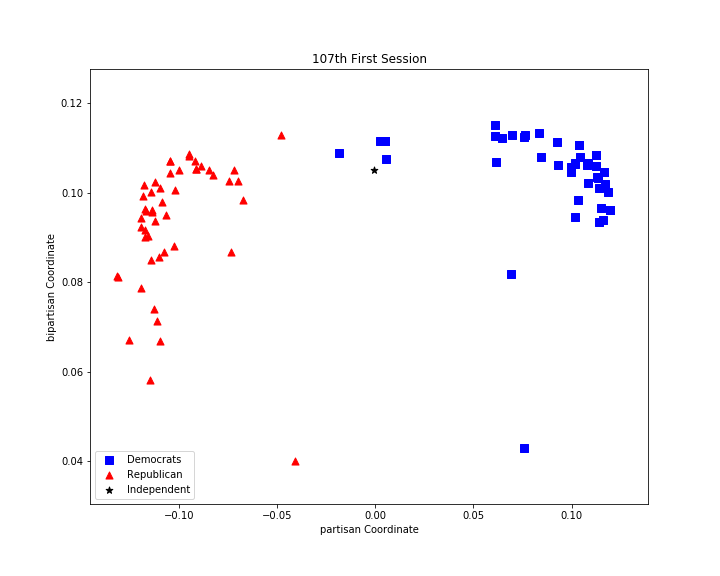
\includegraphics[scale=.5]{107th1.png}
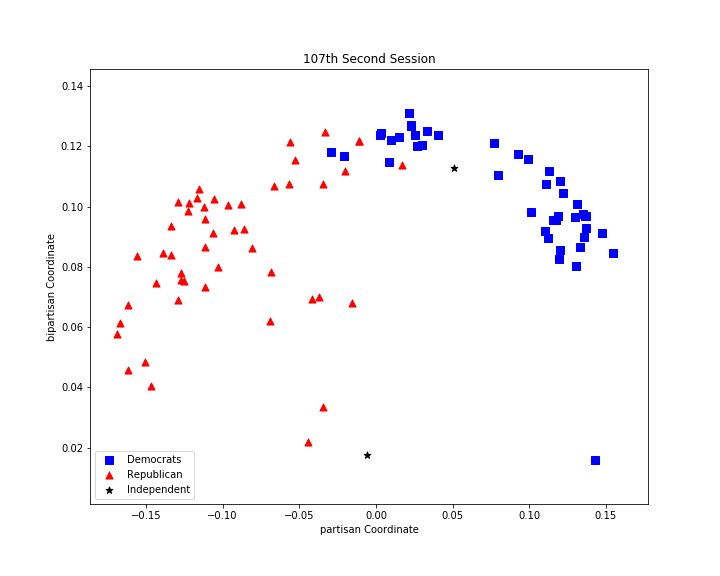
\includegraphics[scale=.5]{107th2.png}
\end{center}
\section{Image Processing Application}
\section{Conclusions}
\newpage
\begin{thebibliography}{9}
\bibitem{Extra}
Martin C. D.,  Porter M. A.. The extraordinary SVD, \textit{Am. Math. Monthly} , 2012, vol. 119 (pg. 838-851)
\bibitem{SVDHowTo}
Web.mit.edu. (2019). \textit{Singular Value Decomposition (SVD) tutorial}. [online] Available at: http://web.mit.edu/be.400/www/SVD/Singular\_ Value\_ Decomposition.htm [Accessed 10 May 2019].
\bibitem{PIL}
Pillow.readthedocs.io. (2019). \textit{Image Module} - \textit{Pillow (PIL Fork) 3.1.2 documentation.} [online] Available at: https://pillow.readthedocs.io/en/3.1.x/reference/Image.html [Accessed 10 May 2019].
\bibitem{Network}
Porter, Mason A., Mucha, Peter J., Newman, M. E. J., and Warmbrand, Casey M. 2005. A network analysis of committees in the U.S. House of Representatives. \textit{Proceedings of the National Academy of Sciences of the United States of America} \textbf{102}: 7057–62.
\end{thebibliography}
\end{document}
